\chapter{结合字词向量的命名实体识别}
\section{基于字词向量结合的特征嵌入与训练}
\subsection{嵌入粒度对命名实体识别的影响}
\label{subsec:analyze}
现有的命名实体识别方法一般基于两个思路,一是以不定长的词为粒度,依赖词性、上下文等特征,对特定的一些词序列进行标注或聚合(分块),最终得到与原文对应的标签序列;二是以字为粒度,依赖字本身的特征进行字符序列的标注。

思路一常见于以传统的基于统计的方法进行的命名实体识别中。
但该方法在实际应用中存在一定缺陷。
首先,基于词粒度的命名实体识别较为依赖分词的结果、词性等先验特征,分词结果的好坏与词性标注的结果将对命名实体识别的结果产生较大的影响;
其次,分词这一任务本身是识别语料中单独成词的序列,而命名实体中存在大量多个词组合而成复合实体,虽然分词的目的并不在于确定命名实体的词边界,但错误的分词结果将会消除命名实体的词边界,在此基础上识别的命名实体必然是错误的;
最后,即便分词结果相对可靠,但由于命名实体本身的结构是多变的,相同的词并不一定总是命名实体,而在训练语料中未被单独分出的词在测试语料中是命名实体,或者测试语料中是命名实体的序列根本未在训练语料中出现过,并且其也并不由训练预料中的某个或某些词组成,那么这样的命名实体就很难被识别出来。

\begin{table}[H]
    \centering
    \caption{基于词的识别部分伪正类和伪负类}
    \begin{tabular}{cccc}
        \toprule
        \multicolumn{2}{c}{False positive} & \multicolumn{2}{c}{False negative}\\
        \midrule
        错识别标签 & 字串 & 未识别标签 & 字串\\
        \cmidrule(lr){1-2}\cmidrule(lr){3-4}
        \multirow{3}{*}{PERSON} & 钟声 & \multirow{3}{*}{PERSON} & 安南 \\
        & 唐诗 & & 简 \\
        & 宋词 & & 老舍\\
        \cmidrule(lr){1-2}\cmidrule(lr){3-4}
        \multirow{2}{*}{LOC} & 苏东坡 & \multirow{2}{*}{LOC}& 梁园\\
        & 关牧村 & & 孟买 \\
        \cmidrule(lr){1-2}\cmidrule(lr){3-4}
        \multirow{2}{*}{ORG} & 复印社 & \multirow{2}{*}{ORG}& 国家银行\\
        & 台湾公司 & & 联合国\\
        \bottomrule
    \end{tabular}
    \label{tab:fp_fn_word}
\end{table}

其原因在于,在进行命名实体识别时,忽略了构成词的字的特征,如“梁孝王刘武……”,由于该序列中存在四个常见的人名姓氏,因此不论是直接分词,还是以姓氏字典作为触发字的识别,在这种情况下都会受到严重干扰,导致最终结果不正确。

总之,本文认为基于词的命名实体识别方法仅在语料规律相对明显,内容相对较为简单,且具备大规模的、成熟的人名、地名和机构名词典或特殊领域知识的情况下,具有很好的效果。
在处理未登录词问题上,还存在较大缺陷。而这里我们尚且仅考虑人名、地名和机构名,并未考虑其他特殊专名、网络新词与领域新词等其他命名实体,因为就命名实体识别而言,存在周期相对较短的部分新词并不作为该任务的关注重点。

\begin{table}[H]
    \centering
    \caption{基于词的识别部分伪正类和伪负类}
    \begin{tabular}{cccc}
        \toprule
        \multicolumn{2}{c}{False positive} & \multicolumn{2}{c}{False negative}\\
        \midrule
        错识别标签 & 字串 & 未识别标签 & 字串\\
        \cmidrule(lr){1-2}\cmidrule(lr){3-4}
        \multirow{3}{*}{PERSON} & 钟声 & \multirow{3}{*}{PERSON} & 成方圆 \\
        & 唐诗 & & 简 \\
        & 宋词 & & 老舍\\
        \cmidrule(lr){1-2}\cmidrule(lr){3-4}
        \multirow{2}{*}{LOC} & 苏东坡 & \multirow{2}{*}{LOC}& 梁园\\
        & 关牧村 & & 孟买 \\
        \cmidrule(lr){1-2}\cmidrule(lr){3-4}
        \multirow{2}{*}{ORG} & 复印社 & \multirow{2}{*}{ORG}& 国家银行\\
        & 台湾公司 & 联合国& \\
        \bottomrule
    \end{tabular}
    \label{tab:fp_fn_word}
\end{table}

思路二是常见于基于神经网络的方法。考虑到以词为
虽然以字为基本元素进行命名实体识别能够取得不错的效果,但其也存在一些问题。
首先,以字符为粒度对语料进行切分,会产生一些过长的字符序列。尽管LSTM在理论上能够接受任意长度的输入序列,但过长的序列会产生层数非常深的LSTM网络,这将使得网络参数量大大增加,训练速度相应降低。
其次,尽管LSTM具有一定的获取长距离上下文语义信息的能力,但若不对时间步的最大值加以限制,BPTT算法在进行误差的反向传播时,还是会面临严重的梯度消失问题,使得模型训练的结果变差。
最后,在神经网络模型中,字的表示来源于根据训练语料获得的字向量或通过大规模未标注语料预训练的字向量。
其信息往往不能完全覆盖预测环境下的语义,部分非命名实的常用字可能也经常出现在命名实体中,而部分非命名实体中的罕用字由于缺乏训练语料的语义信息,往往多被判别为命名实体。

对于序列过长及其导致的梯度消失问题,可行的解决办法包括通过去除停用字、词控制序列长度,制定截断策略在设定的阈值前后切分长序列和对原序列进行采样等方法。本文中所使用训练语料大多不超过250字符,故在以字为基本单位时,序列长度设定不超过250。

而对于同字异义、异字同意等问题,往往来源于歧义。这一部分目前较难从根本上得到解决。

基于上述分析,本文提出一种在模型训练中结合字词向量的方法。该方法能够在降低分词效果对命名实体识别准确率的影响的同时,尽量减少无关的非命名实体的干扰。
\subsection{字向量结合的嵌入和训练}
\label{subsec:combine_word_char}
结合字词向量预训练词嵌入与模型训练的基本思路是,首先对原始语料进行粗切分并进行词性标注,然后取其中所有一级标签为名词词性的单词(包括人名、地名、机构名、一般名词、特殊专名等)切分成单字,保留动词、代词等其他词性的单词。

得到的粗分结果和词性标签,可以作为特征输入模型;也可去除词性标签,降低粗分错误结果产生的噪声对模型的影响。

对预训练向量首先进行全文切分成字,训练字向量;然后同样粗切分为词,训练词向量。最终构建的字词嵌入包含所有字向量和去除单字后的词向量。

训练时,切分以熟语料标注结果为准;测试数据的预处理可使用jieba、hanlp等开源语言处理工具进行处理。需要指出的是,为了减少词性标注中包含的命名实体识别结果,使用分词器进行分词时全部禁用了命名实体识别,并不使用任何附加的命名实体识别词典和领域知识。

本章实验以名词为切分目标,也可根据实际情况,灵活选择需要切分的词性对象。

总体流程可如图所示。
\begin{figure}[H]
    \centering
    \caption{Name}
    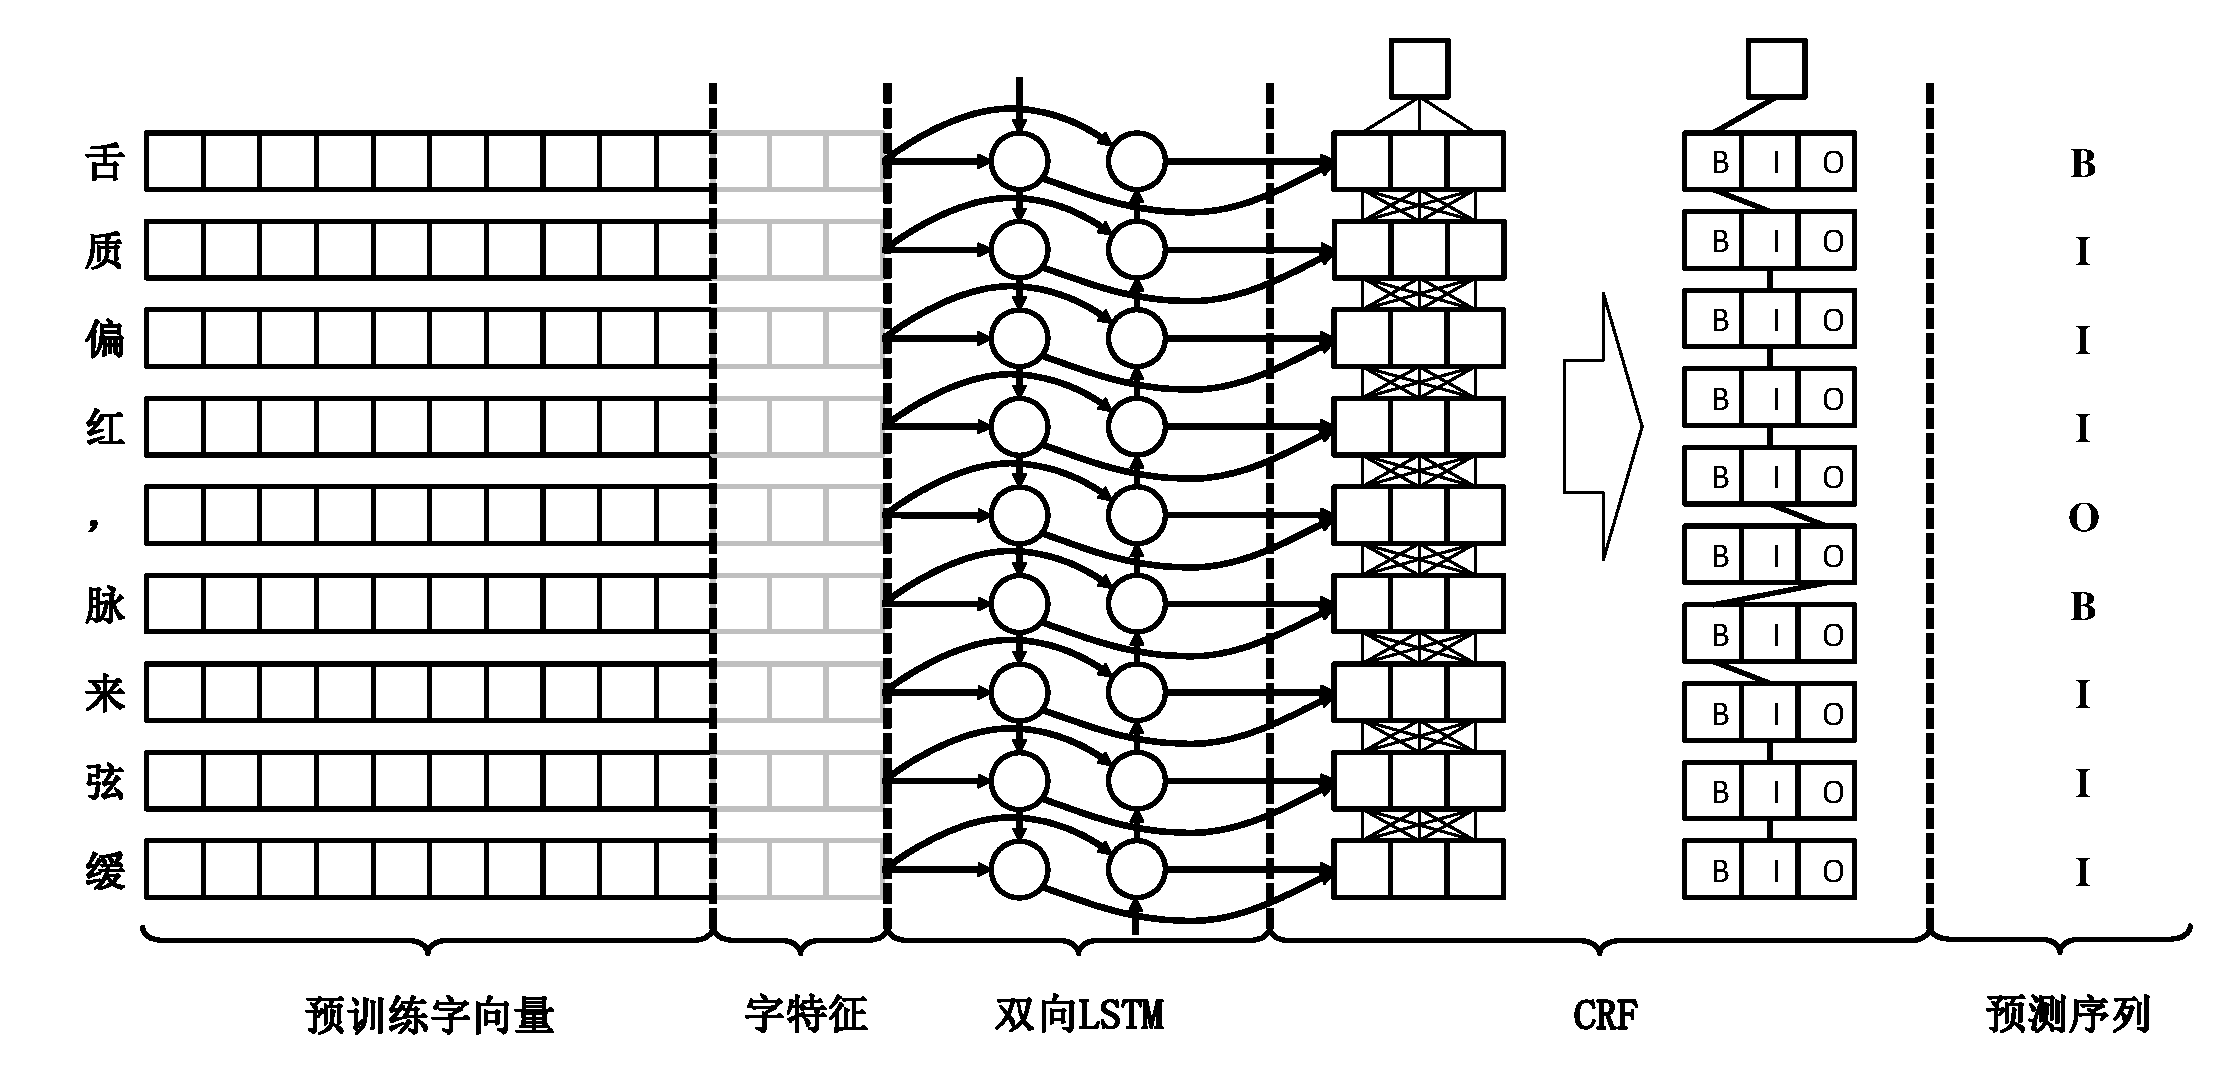
\includegraphics[width=0.8\linewidth]{TCM-NER}
    \label{fig:exp_frame}
\end{figure}

\section{实验设计与数据预处理}
本章实验包括三个部分。首先,先采用第四章介绍的双向LSTM-CRF序列标注框架,分别建立使用字向量、词向量作为训练数据的的基线模型,并在这一部分考察使用不同LSTM实现对公开领域语料命名实体识别的效果,对比不同模型对词性特征的依赖程度。

其次,选取在基线实验部分表现较好的实现作为进一步的实验框架,增加结合字词向量作为训练数据的是实验组,调整模型参数,采用五折交叉验证获取多组实验数据,对得到的准确率、召回率求平均值作为实验的最终结果。

最后,在减少词性特征的条件下重复实验,对比分析不同模型在不依赖词性的情况下进行命名实体识别的效果。


实验数据的准备包含两部分:字词向量嵌入和训练语料预处理。

字词向量的嵌入采用中文维基百科语料库,总大小约1.5G。使用Word2Vector的实现之一Gensim进行字词向量的训练。
其中,对字进行训练是针对命名实体,可能包含较多不常用字,因此字向量的获取采用Hierachical Softmax模型,上下文窗口设置为5,采样率为$10^-4$,最小词频设置为1,获取所有字的嵌入。
对词向量的训练针对常见词,模型采用Negative Sampling,最小词频设置为5,过滤掉罕见词。
最终获取的词向量为300维,其中字向量22884个,词向量544568个。

训练语料来源于人民日报,包含1998年1至6月经人工标注的语料。构建五折交叉实验数据时,每次取2-6月其中一月数据作为测试集,其他数据作为训练集,进行开放测试。

原始语料格式如下:

\begin{verbatim}
本报/r  哈尔滨/ns  1月/t  1日/t  电/n  记者/n  董/nr  伟/nr
报道/v  :/w  顶/v  着/u  寒风/n  ,/w  黑龙江省/ns  各级/r
领导/n  组成/v  若干/m  慰问/vn  小组/n  ,/w  在/p  节日/n
期间/f  深入/v  到/v  厂矿/j  车间/n  ,/w  为/p  困难/a  职工/n
送/v  去/v  党/n  的/u  温暖/an  。/w
\end{verbatim}

预处理过程中根据已经标注好的词性,按照节\ref{subsec:combine_word_char}思路进行如下处理:
\begin{enumerate}
    \item 去除特殊符号、空标注等非法字符
    \item 去除l、i等与本文任务无关的组合词标签
    \item 合并组合命名实体,根据词性标签nr, ns, nt分别标注命名实体及其组成元素。标注模式如表x所示
    \item 合并所有名词类词性标签,去除人名、地名、机构名的二级类别标签,全部用一级类别n取代
    \item 分别生成字、词和字词结合的训练语料与测试语料
    \item 去除所有词性标签,作为对比实验语料
\end{enumerate}

对人民日报原始语料进行实体标签标注时采用BIO模式,标签设置如下表所示。

\begin{table}[H]
    \centering
    \caption{标注模式}
    \begin{tabular}{ll}
        \toprule
            BIO标签集\\
        \midrule
        B-PER & 人名起始及单字(词)人名 \\
        I-PER & 人名中间字词 \\
        B-LOC & 地名起始及单词地名 \\
        I-LOC & 地名中间字词 \\
        B-ORG & 机构名起始及单词机构名 \\
        I-ORG & 机构名中间字词 \\
        O & 非命名实体\\
        \bottomrule
    \end{tabular}
\end{table}

实验平台基于Ubuntu 16.04LTS,CPU为Intel I5 8600K CPU,GPU 为nVidia GeForce GTX 1070Ti,内存为16G。双向LSTM-CRF序列标注框架的实现基于TensorFlow-GPU 1.6.0,Python版本为3.5。
所有实验均使用GPU加速,CUDA版本为8.0, cuDNN版本为7.0。

模型的超参数设置如下:
\begin{table}[H]
    \centering
    \caption{参数列表}
    \begin{tabular}{ll}
        \toprule
        \multicolumn{2}{c}{模型超参数设置} \\
        \midrule
        batch\_size & 512(字嵌入)/800(词嵌入) \\
        隐藏层单元数量 & 256\\
        全局drop\_out\_rate & 0.5 \\
        l2正则化参数 & 0.01 \\
        初始学习率 & 0.002 \\
        早停等待epoch数 & 3\\
        序列最大长度 & 250(字嵌入)/120(词嵌入)\\
        \bottomrule
    \end{tabular}
\end{table}
其中,batch\_size由于显存限制,最大设置为表中数值;实际选择结果最优的参数重复实验。训练集与验证集的比例为9:1。

\section{实验结果与分析}
与章节\ref{sec:tcm-pfr}中提到的评价标准不同的是,本节数据来源于公共领域数据集,对人名、地名和机构名的界定相较中医症状术语而言更为明确,且语料本身质量较高,能够明确地确定单个实体。
故本节以整个命名实体识别结果作为评价对象。模型识别结果与实际结果完全一致则可归为正类,否则即为负类。具体表示为:
\begin{align}
    Precision = \frac{True Positive}{Predict Size} \times 100\%
    Recall = \frac{True Positive}{Entity Size} \times 100\%
    F-measure = \frac{2\times Precision \times Recall}{Precision + Recall}
\end{align}
其中$True Positive$指完全识别正确的实体数,$Predict Size$指识别的实体数,$Entity Size$指实际存在的实体数。

需要指出的是,本文进行的五折交叉实验,实验数据情况与文献\citepns{吴友政2006汉语问答系统关键技术研究}中的情况类似。
本文考虑到人民日报语料本身的性质,其中存在大量命名实体,其内容和出现的上下文在整个语料集中具有较好的一致性,故可能与其他语料存在一定差异,特此提出。
但这并不影响方法的效果的对比。

首先,在只以字嵌入作为特征的情况下,对比不同LSTM实现下,命名实体识别结果的差异。
\begin{table}[H]
    \centering
    \caption{实验一:以字嵌入作为特征}
    \begin{tabular}{cccccccccc}
        \toprule
            \multirow{2}{*}{Cell} &\multicolumn{3}{c}{PERSON} &\multicolumn{3}{c}{LOC} &\multicolumn{3}{c}{ORG}\\
            \cmidrule(lr){2-4} \cmidrule(lr){5-7} \cmidrule(lr){8-10}
            & P & R & F1 & P & R & F1 & P & R & F1\\
        \midrule
        LSTM(baseline) & 95.73 & 93.54 & 94.62 & 93.40 & 93.07 & 93.24 & 89.81 & 92.85 & 91.31\\
        LSTM(peep-hole) & 95.61 & 93.80 & 93.23 & 92.97 & 93.49 & 93.23 & 90.60 & 92.19 & 91.39\\
        GRU & 95.21 & 94.13 & 94.67 & 93.46 & 93.64 & 93.55 & 90.46 & 92.75 & 91.59\\
        CIFG  & 96.26 & 93.16 & 94.68 & 93.33 & 93.57 & 93.45 & 90.60 & 92.87 & 91.72\\
        \bottomrule
    \end{tabular}
    \label{tab:tab1}
\end{table}
实验数据表明,在仅使用字特征的情况下,

基于词向量的命名实体识别。
\begin{table}[H]
    \centering
    \caption{实验二:基于词嵌入的命名实体识别}
    \begin{tabular}{cccccccccc}
        \toprule
            \multirow{2}{*}{Cell} &\multicolumn{3}{c}{Overall} &\multicolumn{3}{c}{B} &\multicolumn{3}{c}{I}\\
            \cmidrule(lr){2-4} \cmidrule(lr){5-7} \cmidrule(lr){8-10}
            & F1 & R & P & F1 & R & P & F1 & R & P\\
        \midrule
            LSTM & *0.724 & 0.621 & 0.866 & 0.736 & 0.635 & 0.874 & 0.718 & 0.600 & 0.894\\
            (baseline) & 0.756 & 0.675 & 0.860 & 0.763 & 0.685 & 0.862 & 0.753 & 0.653 & 0.889\\
            LSTM & *0.748 & 0.691 & 0.815 & 0.746 & 0.689 & 0.812 & 0.748 & 0.670 & 0.848\\
            (peep-hole) & 0.763 & 0.699 & 0.839 & 0.748 & 0.685 & 0.824 & 0.769 & 0.687 & 0.873\\
            \multirow{2}{2cm}{GRU} & *0.754 & 0.717 & 0.796 & 0.738 & 0.689 & 0.794 & 0.761 & 0.698 & 0.835\\
                                 & 0.762 & 0.708 & 0.825 & 0.758 & 0.707 & 0.816 & 0.764 & 0.687 & 0.861\\
            \multirow{2}{2cm}{CIFG} & *0.742 & 0.664 & 0.839 & 0.749 & 0.662 & 0.863 & 0.738 & 0.640 & 0.872\\
                                  & 0.780 & 0.735 & 0.832 & 0.762 & 0.707 & 0.826 & 0.788 & 0.725 & 0.863\\
        \bottomrule
    \end{tabular}
    \label{tab:tab1}
\end{table}
由表可见,词嵌入与基于神经网络的序列标注框架的适应性很差,分词的结果与标注模式相差较大,导致命名实体识别的准确率、召回率都很低,这表明在真实条件下依赖分词结果进行命名实体识别可行性较低。
其分词标注如果与训练模型的标注标准不统一,会在嵌入和训练两个阶段导致命名实体识别效果低下:
一是分词结果若在预训练向量中未出现,则模型将在预测时随机初始化嵌入向量,将该词作为未登录词处理。这样就难以利用组成该词的字向量进行识别。
二是若作为未登录词输入模型,则模型将词所在上下文对其标签进行预测。若分词结果不一致,其上下文必然存在较大差异。而在同样以词为基本单位的训练数据中,更难存在上下文类似的训练场景。
这导致第一阶段造成的影响进一步被放大,最终效果很不理想。

去除词性影响后..(一顿分析)

可见在两种不同预训练嵌入下,xxx在命名实体识别上取得了更佳的性能。

使用字词向量结合的嵌入模型试验结果
\begin{table}[H]
    \centering
    \caption{实验五:字词向量结合命名实体识别结果}
    \begin{tabular}{cccccccccc}
        \toprule
            \multirow{2}{*}{Cell} &\multicolumn{3}{c}{Overall} &\multicolumn{3}{c}{B} &\multicolumn{3}{c}{I}\\
            \cmidrule(lr){2-4} \cmidrule(lr){5-7} \cmidrule(lr){8-10}
            & F1 & R & P & F1 & R & P & F1 & R & P\\
        \midrule
            LSTM & *0.724 & 0.621 & 0.866 & 0.736 & 0.635 & 0.874 & 0.718 & 0.600 & 0.894\\
            (baseline) & 0.756 & 0.675 & 0.860 & 0.763 & 0.685 & 0.862 & 0.753 & 0.653 & 0.889\\
            LSTM & *0.748 & 0.691 & 0.815 & 0.746 & 0.689 & 0.812 & 0.748 & 0.670 & 0.848\\
            (peep-hole) & 0.763 & 0.699 & 0.839 & 0.748 & 0.685 & 0.824 & 0.769 & 0.687 & 0.873\\
            \multirow{2}{2cm}{GRU} & *0.754 & 0.717 & 0.796 & 0.738 & 0.689 & 0.794 & 0.761 & 0.698 & 0.835\\
                                 & 0.762 & 0.708 & 0.825 & 0.758 & 0.707 & 0.816 & 0.764 & 0.687 & 0.861\\
            \multirow{2}{2cm}{CIFG} & *0.742 & 0.664 & 0.839 & 0.749 & 0.662 & 0.863 & 0.738 & 0.640 & 0.872\\
                                  & 0.780 & 0.735 & 0.832 & 0.762 & 0.707 & 0.826 & 0.788 & 0.725 & 0.863\\
        \bottomrule
    \end{tabular}
    \label{tab:tab1}
\end{table}
以人民日报1998年2月标注语料为例,其中包含词性标签1149582个,其中名词为309909个。在非名词标签中,两字以上词有325034个,包含字符数总计708000以上。
若以字嵌入进行识别,则整个语料将增加70余万行,相应训练模型时最大序列长度也将提升。

综合对比各模型的性能:
\begin{table}
    \centering
    \begin{tabular}{cccc}
        \toprule
        \multicolumn{4}{c}{不同嵌入粒度和词性特征的识别效果}\\
        \midrule
        嵌入粒度 & P  & R  & F1\\
        \midrule
        char & & &\\
        char\_pos & & &\\
        word & & &\\
        word{pos} & & &\\
        char+word & & &\\
        char+word\_pos& & &\\
    \end{tabular}
    \caption{<+Caption text+>}
    \label{tab:<+label+>}
\end{table}


最后,本文认为模型训练效率也是一个考察方法性能的重要指标。在实验过程中,我们记录了各次实验中训练模型所需的时间,按照模型嵌入粒度、是否使用词性特征两个维度分别对训练模型的平均时间进行对比,结果如表\ref{tab:train_time}所示。

\begin{table}
    \centering
    \begin{tabular}{ccc}
        嵌入粒度 & \multicolumn{2}{c}{消耗时间(s)}\\
        \midrule
        char  & 10433\\
        char\_pos & 1000\\
        word  & 1000\\
        word\_pos  & 1000\\
        word\_char  & 5993\\
        word\_char\_pos  & 1000\\
    \end{tabular}
    \caption{<+Caption text+>}
    \label{tab:<+label+>}
\end{table}

通过结果可以看出,字向量的平均训练时间都在1000s以上,单个epoch训练时间在210s左右,实际训练过程中单个模型训练epoch在20以上时,验证集上的损失才能收敛;这时batch-size已经设置为显存能够允许的最大值。这在一定程度上验证了节\ref{subsec:analyze}对字嵌入训练模型的缺点的分析,由于此时粒度细,输入序列相应变长,导致模型参数量和计算量大大增加,训练耗时也增加不少。
这在更大规模的数据集上会更加明显。

相对而言词向量与字词向量结合能够节省更多的时间。但词向量在该模型下识别效果很差,而字词向量结合试图寻找二者之间的平衡点,取得了相对不错的平衡性。

综合比较下,字词向量结合的训练方法能够在不损失很多精度的同时,提升模型训练效率,并且在部分实验指标中达到了与字向量结果持平或稍好的效果,具有一定实际应用价值。

\section{本章小结}
本章在传统基于字、词粒度进行命名实体识别的基础上,考察了命名实体识别错误发生的特点,提出了融合两种粒度对字词嵌入进行混合的思路,并基于此思路对标注框架中预训练词向量与训练、测试数据进行预处理。在此基础上,对比了多粒度训练的模型在不同LSTM实现上的效果。同时,还针对词性特征对命名实体识别结果的影响,对比了不同粒度嵌入下有无词性特征的识别效果。

本章针对预训练词向量和训练、测试语料处理这一环节,提出了可行的整合字词向量的思路,并在实际应用中取得了一定的效果。
